\section*{Этап 1}

\addcontentsline{toc}{section}{Этап 1}

\subsection*{Описание предметной области}

Существует вселенная, где герои живут уже тысячи лет. Новые герои поставляются корпорацией и имеют разный запас здоровья.\\

Есть пользователи, те инопланетные существа, которые покупают героев и зарабатывают на боях своих героев.\\

Герои деруться песнями, с каждым героем корпорация поставляет в комплекте несколько песен, которые постепенно открываются с растущим опытом героя. Песня может измельчаться на ноты, своеобразные "патроны", которые наносят урон.

\addcontentsline{toc}{subsection}{Описание предметной области}

\subsection*{Описание бизнес процессов}

\addcontentsline{toc}{subsection}{Описание бизнес процессов}

При первом входе в игру дается 1000 золота и 0 опыта.\\
    
Игроки покупают героев. У игроков есть валюта, чтобы платить за героев, у героев есть цена.\\

После покупки героев, игроки могут выставлять по одному герою на поле битвы. Участие может принимать несколько игроков и ходят по очереди, тот кто ходит первый определяется рандомом.\\

Перед сражением игрок может выбрать эффект, с которым будет ходить его герой всю битву и песню, которую будет в этой битве исполнять. \\

Герои дерутся между собой песнями. Песни имеют минимальный уровень опыта, который должен иметь герой, чтобы начать их использовать. То есть песни разблокируются постепенно.\\
    
После того, как разыгралось сражение и есть выигравший герой. У всех игроков отнимается 100 золота перераспределяется в пропорциях равных, кол-ву нанесённого урона. \\

Если деньги заканчиваются, игроку необходимо либо купить игровые деньги за валюту, либо открыть лутбокс, который выдаётся каждому игроку раз в день. \\

Есть список пользователей в онлайне, пользователь приглашает другого пользователя в драку и тот либо отклоняет либо принимает заявку на битву.


\subsection*{Сущности}

\addcontentsline{toc}{subsection}{Сущности}

\begin{itemize}
\item \textbf{Стержневые сущности}
\begin{enumerate}
    \item Песня(id, имя, порог\_опыта, id\_героя, урон)
    \item Игрок(id, имя, баланс, статус\_онлайна, хэш\_пароля)
    \item Персонаж(id, имя, цена, стоимость, здоровье, путь\_к\_аватарке)
    \item Эффект(id, название, цена, выносливость, сила, удача, конституция)
    \item Драка(id, время\_начала, id\_локации)
\end{enumerate}

\item \textbf{Ассоциативные сущности}
\begin{enumerate}
    \item Ходы\_в\_драке(номер\_хода, id\_драки, id\_атакующего, id\_атакуемого, урон)
    \item Сделка(id\_игрока, плата)
    \item Сделка\_по\_герою(id\_сделки, id\_героя)
    \item Сделка\_по\_эффекту(id\_сделки, id\_эффекта)
    \item Участник\_драки(id, id\_драки, id\_эффекта\_в\_драке, id\_используемой\_песни, id\_героя, полученный\_опыт, полученное\_золото, позиция)
    \item Герой(id, опыт, id\_персонажа, id\_игрока)
\end{enumerate}

\item \textbf{Характеристические сущности}
\begin{enumerate}
    \item Локация(id, название)
\end{enumerate}
\end{itemize}

\section*{Этап 2}

\addcontentsline{toc}{section}{Этап 2}

\subsection*{Нарисовать ER-диаграмму предметной области}

\addcontentsline{toc}{subsection}{Нарисовать ER-диаграмму предметной области}

\begin{figure}[H]
	\begin{center}
		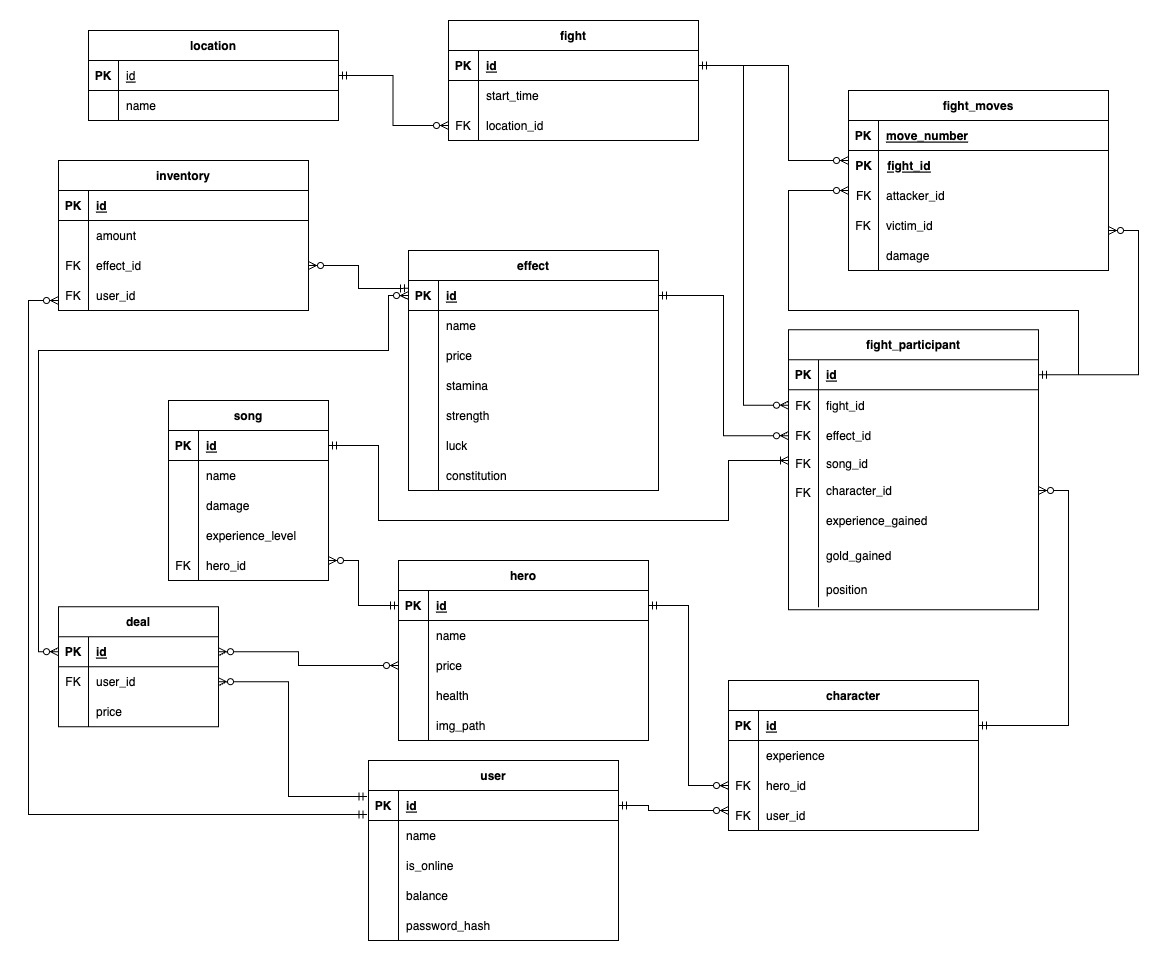
\includegraphics[scale=0.46]{images/ER.jpg}
		\caption{ER-диаграмма предметной области}
	\end{center}
\end{figure}

\subsection*{На основе ER-модели построить даталогическую модель}

\addcontentsline{toc}{subsection}{На основе ER-модели построить даталогическую модель}

\begin{figure}[H]
	\begin{center}
		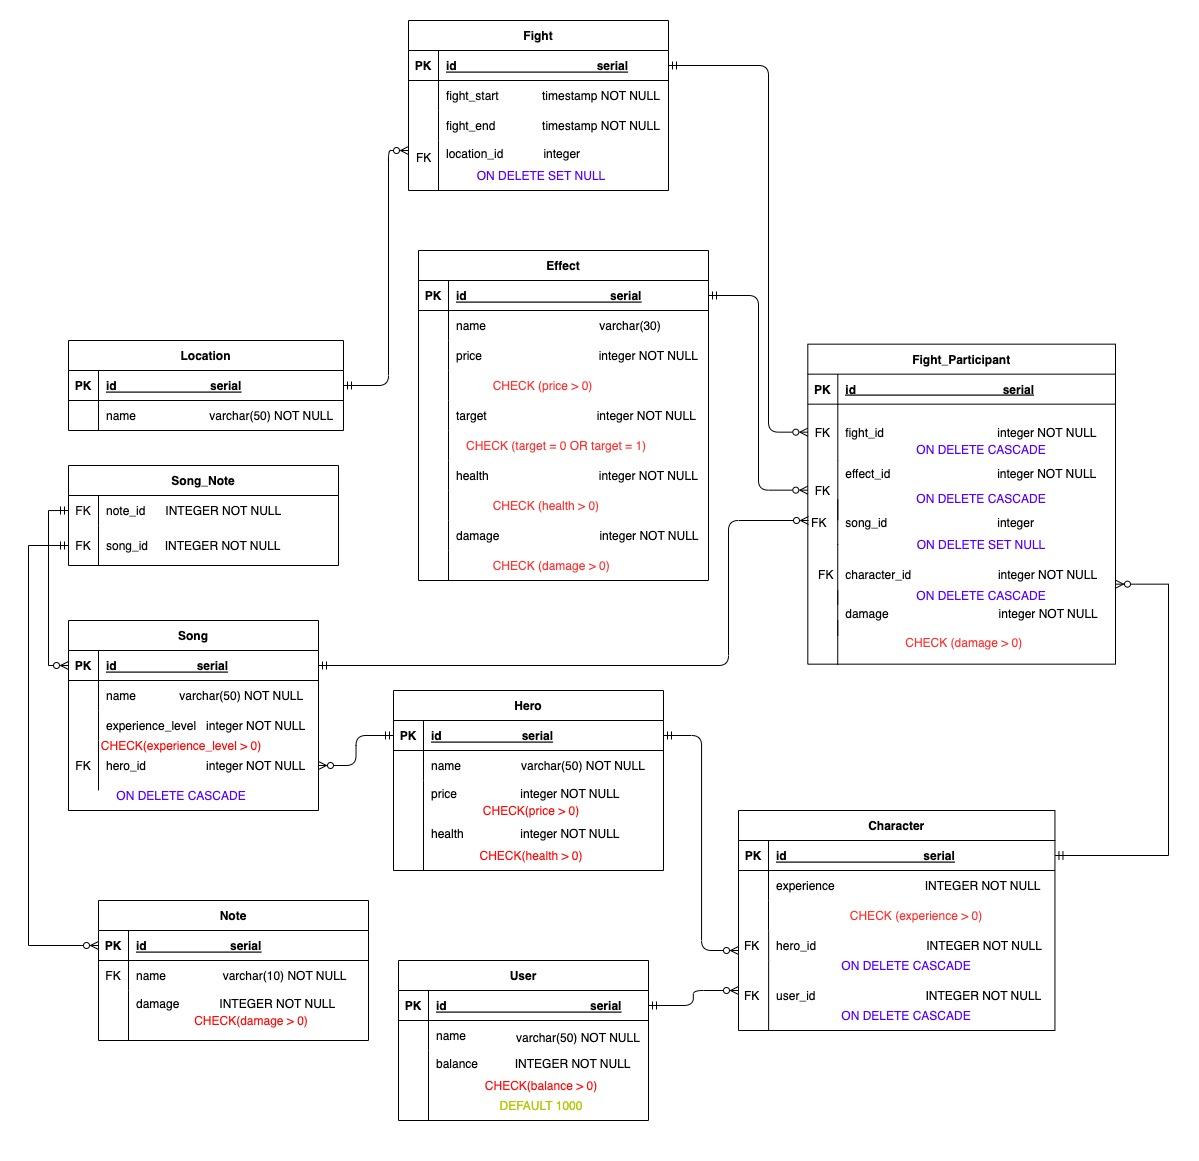
\includegraphics[scale=0.44]{images/Datalogical.jpg}
		\caption{Даталогическая модель}
		\label{pic:pic_name} % название для ссылок внутри кода
	\end{center}
\end{figure}

\newpage

\section*{Этап 3}

\addcontentsline{toc}{section}{Этап 3}

\subsection*{Сделать скрипты для создания и удаления базы данных}

\addcontentsline{toc}{subsection}{Сделать скрипты для создания и удаления базы данных}

\begin{enumerate}
    \item buy\_hero(user\_id, hero\_id, sum) 
    - юзер покупает героя, создаем сущность Character

    \item get\_online\_list() -> List<User>
    - выводим список юзеров, которые находятся в сети

    \item inter\_fight(location\_id, song\_id\_0, song\_id\_1, hero\_id\_0, hero\_id\_1, effect\_0, effect\_id\_1, user\_id\_0, user\_id\_1) -> fight\_id
    - Создаёт запись в fight с начальным временем, создаёт запись в fight\_participant с пользователем, добавляет битву в него 

    \item add\_fight\_participant(song\_id, character\_id, effect\_id, fight\_id)

    \item finish\_fight(fight\_id, character\_id) -> None
    - Поставить ссылку на победителя в битве

    \item get\_available\_songs(character\_id) -> song\_id
    - находит доступные для выбора песни
    
    \item get\_effects() -> List<Effect>
    - получить все доступные эффекты 
    
    \item get\_locations() -> List<Location>
    - получить все локации

    \item get\_fight\_participants(fight\_id) -> List<Fight\_Participant>
    - Получить список участников сражения

    \end{enumerate}

\subsection*{Добавить в базу данных триггеры для обеспечения комплексных ограничений
целостности}

\addcontentsline{toc}{subsection}{Добавить в базу данных триггеры для обеспечения комплексных ограничений
целостности}

\begin{enumerate}
    \item On update fight 
    - Берем бабки и опыт с програвшего, берем с победителя и по бизнес логике перераспределяем через 2 join'a на user'a

    \item On buy hero
    - При вставке новой сущности в character снимаем деньги с user'a

    \item On update fight\_participant
    - Сверяет damage и определяет победителя если он >= со здоровьем, то он умер
    
\end{enumerate}ww